\section{Numerical experiments}
\label{sec:results}

\subsection{Setup}
\label{sec:setup}

\paragraph{Potentials} In one dimension we use the harmonic oscillator
$V=\tfrac12x^2$ on $[-6,6]$, the infinite square well on $[0,1]$, and a finite
square well of depth $V_0=50$ and half-width $1$ on $[-8,8]$. The first two
have closed-form spectra, which we use only to construct training references
and to label the runs; the certificate never sees them. In two dimensions we
use $V=\tfrac12(x^2+y^2)$ on $[-3,3]^2$, the box $[0,1]^2$, and the
non-separable potential $V=\tfrac12(x^2+y^2)+\tfrac12x^2y^2$ on $[-3,3]^2$,
for which no closed form is used at all: the certificate does not need one and
neither does the reference, which is the dense LAPACK solve described under
\emph{References} below.

\paragraph{Networks and training} One-dimensional runs use an MLP of width
64 and depth 3 with Fourier features, $10^4$ epochs of Adam, and a grid of
2001 points; two-dimensional runs use width 64, depth 4, no Fourier features,
6000 epochs and an $81\times81$ grid. The loss is \eqref{eq:loss}. Three seeds
(0, 1, 2) are run for every potential; all reported ranges are over seeds.

\paragraph{References} Every enclosure is compared against a value obtained
independently of both the network and the certificate: in 1D by LAPACK's
symmetric tridiagonal solver, evaluated as the Rayleigh quotient of the
returned vector (the raw LAPACK eigenvalue has absolute error of order
$\varepsilon\norm{\Hh}$, from $7\times10^{-12}$ on the finite-well grid to
$2\times10^{-9}$ on the box grid, at least as large as the narrowest widths
being tested); in
2D by a dense LAPACK decomposition of the full $6241\times6241$ matrix. ARPACK
is used in 2D only to propose interval endpoints; it agrees with the dense
reference to all ten printed digits and is never the reference itself. The
reference is used for validation only; it is never an input to the
certificate.

\subsection{One-dimensional ground states}
\label{sec:1d}

Table~\ref{tab:1d} summarises the nine ground-state runs with the
leakage-free (Rayleigh-quotient) residual.

\begin{table}[t]
\centering
\small
\setlength{\tabcolsep}{2pt}
\begin{tabular}{lccc}
\toprule
 & Harmonic & Infinite well & Finite well \\
\midrule
raw cert. & 2/3 & 2/3 & 3/3 \\
$|E_f-\lambda_h|$ & $1.6\times10^{-6}$--$7.4\times10^{-5}$ & $3.7\times10^{-14}$--$1.8\times10^{-13}$ & $(1.3\text{--}7.7)\times10^{-4}$ \\
width, raw & $0.143$--$0.65$ & $(5.9\text{--}6.2)\times10^{-4}$ & $0.553$--$2.76$ \\
width, filtered & $2.7\times10^{-5}$--$9.3\times10^{-4}$ & $9.9\times10^{-12}$ & $0.374$--$0.729$ \\
angle bound & $3.7\times10^{-3}$--$2.2\times10^{-2}$ & $(7.3\text{--}7.5)\times10^{-10}$ & $0.56$--$0.835$ \\
contains $\lambda_h$ & 3/3 & 3/3 & 3/3 \\
\bottomrule
\end{tabular}

\caption{One-dimensional ground states, three seeds per potential, 2001-point
grid, $10^4$ epochs. ``raw cert.'' is the number of seeds for which the
unfiltered network output is certifiable. Widths and angle bounds are from the
filtered certificate; ``contains'' counts the enclosures that contain the
independently computed $\lambda_h$.}
\label{tab:1d}
\end{table}

All nine enclosures contain $\lambda_h$, and after filtering all nine runs are
certifiable. The raw certification rate is $7/9$: two networks produce
outputs whose residual is too large relative to the spectral gap for the
Temple condition \eqref{eq:templecond} to hold, which is exactly the situation
in which an unfiltered claim would have to be withheld.

The three potentials separate sharply.
\begin{itemize}
\item \emph{Harmonic.} Certified widths $2.7\times10^{-5}$ to
  $9.3\times10^{-4}$, angle bounds $3.7\times10^{-3}$ to
  $2.2\times10^{-2}$~rad against true angles of $9\times10^{-4}$ to
  $5\times10^{-3}$~rad. The
  enclosure is between 5 and 19 times wider than the true error---usable, and
  the only potential where it is.
\item \emph{Infinite well.} Width $9.9\times10^{-12}$, i.e.\ at the
  round-off floor of the interval endpoints. This is not evidence that the
  network is accurate to $10^{-11}$; it is evidence that after filtering the
  network output is a single sine mode, and the residual of that mode is
  limited only by the arithmetic. We report it as a validation of the
  mechanism, not as a precision claim.
\item \emph{Finite well.} Widths $0.37$--$0.73$ and angle bounds up to
  $0.84$~rad, against a true energy error of $1.3$--$7.7\times10^{-4}$ and a
  true angle of $10^{-3}$--$3\times10^{-3}$~rad. The enclosure is correct and
  useless: the ratio of certified width to true error is $10^{3}$. The reason is structural---the kink at
  $|x|=1$ makes the discrete eigenvalue converge at first order, and the
  network's short-wavelength error near the interface is indistinguishable,
  from the inside, from a genuine high-wavenumber component of the exact
  eigenfunction. No amount of training removes the ambiguity; only a
  different discretization (or a bound that uses regularity) would.
\end{itemize}

This spread is the main practical message of the paper: a certificate is not
uniformly tight, and the ratio between certified width and true error is
itself a quantity that must be reported.

\subsection{What the filter does}
\label{sec:filter-results}

Figure~\ref{fig:filter}(a) shows the certified width as a function of the
truncation order $K$ for one run per potential. The harmonic curve has the
shape of a bias--variance trade-off: at $K=8$ the truncation discards
legitimate structure and the width is $0.31$; the width falls by four orders
of magnitude to $3.0\times10^{-5}$ at $K=15$, stays flat through $K=20$, and
then grows steadily as noise modes re-enter the residual, reaching $0.59$ at
$K=1500$. The minimum is selected without any reference, from the certificate
alone, and it coincides with the point beyond which the residual is dominated
by components that do not affect the energy. For the infinite well the
minimum is at $K=1$ and the curve is monotone increasing: the exact state is
the first sine mode and every additional mode is noise. For the finite well
the minimum is broad and shallow ($K=600$, width $0.37$), again reflecting the
inability of the basis to separate interface error from physics.

The relative $L^2$ change caused by the filter is
$4\times10^{-6}$--$1.6\times10^{-3}$ over the eighteen runs of the main sweep
(and at most $7\times10^{-3}$ anywhere in the leakage audit), so the object
being certified is not a different function in any
meaningful sense; what is removed is a high-frequency tail that carries most
of the residual and almost none of the energy.

\subsection{Leakage audit}
\label{sec:leak-results}

Table~\ref{tab:leakage} compares four training variants that differ only in
where the energy in the residual comes from. The Rayleigh-quotient variant
\eqref{eq:loss} uses no external information. The learnable-scalar variant
optimises $E_\theta$ jointly with the network. The reference variant uses the
exact energy---a leak, since that is precisely the quantity being predicted.
The deflation variant projects out analytic reference states to reach excited
states---also a leak.

\begin{table}[t]
\centering
\small
\setlength{\tabcolsep}{4pt}
\begin{tabular}{lccccc}
\toprule
Residual energy & raw & filt.\ contains & med.\ $|\Delta E|$ & med.\ width & max width \\
\midrule
Rayleigh (no leak) & 7/9 & 9/9 & $4.9\times10^{-6}$ & $3.0\times10^{-5}$ & $0.729$ \\
Learnable scalar $E_\theta$ & 5/9 & 9/9 & $7.2\times10^{-6}$ & $4.9\times10^{-5}$ & $2.72$ \\
Reference $E$ (leaky) & 8/9 & 9/9 & $6.4\times10^{-6}$ & $2.6\times10^{-5}$ & $0.628$ \\
Deflation (leaky) & 0/3 & 3/3 & $0.109$ & $0.218$ & $0.486$ \\
\bottomrule
\end{tabular}

\caption{Leakage audit: same architecture, $10^4$ epochs, only the energy in
the residual changes. Median $|\Delta E|$ is measured against the discrete
reference; widths are after filtering.}
\label{tab:leakage}
\end{table}

Three observations. First, the three variants that differ only in the energy
in the residual are within a factor of two of each other on the smooth
potentials, so a single-potential comparison would have found nothing; the
deflation variant trains a different state and is not comparable (median
$|\Delta E|=0.11$ against $10^{-5}$). Second, on the finite well the reference variant is markedly better
($0.34$--$0.63$) than the learnable-scalar variant ($1.87$--$2.72$), because a
learnable scalar does not converge within $10^4$ epochs on a potential whose
energy is $-48.97$ (it stalls near $-9.7$); the leak buys accuracy by
supplying the very quantity that is hard to learn. Third, the Rayleigh variant
recovers most of the leak's advantage without the leak ($0.37$--$0.73$),
which is why it is the protocol's default.

A fourth observation concerns what an energy error hides. On the
infinite-well grid, where an eigenfunction is a single sine mode, the
learnable-scalar variant reaches $|\eta-\lambda_h|=2.6\times10^{-7}$ in one
seed---the Rayleigh quotient of the raw output, not of the filtered one---while
the residual of that output is $0.53$. The certificate accepts the run, the
enclosure before filtering is $0.30$ wide, $10^{6}$ times the true error, and
the angle bound is $0.56$~rad: the energy is right to seven digits and the
eigenfunction is located only to $32^\circ$. This is the case quoted in
Section~\ref{sec:intro}.

The honest conclusion of the audit is narrower than ``the certificate detects
leakage''. The certificate describes the quality of a function; it cannot
determine where a number came from. What it does provide is a fixed
measurement scale: the audit becomes a controlled experiment, and the
statement ``method A is better than B'' can be checked against a certified
width rather than against a reference the method may have seen.

\subsection{Multiple states}
\label{sec:multistate}

Reaching excited states requires an extra mechanism, because the residual
functional is minimized by the ground state. We use deflation: after training
the ground state with seed $s$, the network for state $n$ is projected at
every step onto the orthogonal complement of the previously trained states of
the \emph{same seed}---never onto analytic references. The projection is exact
to machine precision ($|\langle\phi,\psi\rangle|\le2\times10^{-16}$ after
re-projection).

\begin{table}[t]
\centering
\small
\footnotesize
\setlength{\tabcolsep}{4pt}
\begin{tabular}{lcccccc}
\toprule
Potential & $n$ & raw & match & contains $n$ & med.\ $|\Delta E|$ & med.\ width \\
\midrule
Finite well & 0 & 3/3 & 3/3 & 3/3 & $6.8\times10^{-4}$ & $0.652$ \\
Finite well & 1 & 3/3 & 3/3 & 3/3 & $3.6\times10^{-4}$ & $0.426$ \\
Finite well & 2 & 3/3 & 3/3 & 3/3 & $6.7\times10^{-4}$ & $0.523$ \\
Harmonic & 0 & 2/3 & 3/3 & 3/3 & $4.9\times10^{-6}$ & $3.0\times10^{-5}$ \\
Harmonic & 1 & 2/3 & 2/3 & 2/3 & $3.7\times10^{-6}$ & $3.6\times10^{-5}$ \\
Harmonic & 2 & 3/3 & 2/3 & 2/3 & $1.2\times10^{-6}$ & $4.7\times10^{-5}$ \\
Infinite well & 0 & 2/3 & 3/3 & 3/3 & $7.1\times10^{-14}$ & $9.9\times10^{-12}$ \\
Infinite well & 1 & 3/3 & 3/3 & 3/3 & $4.2\times10^{-10}$ & $7.2\times10^{-10}$ \\
Infinite well & 2 & 3/3 & 3/3 & 3/3 & $1.2\times10^{-9}$ & $2.6\times10^{-9}$ \\
\bottomrule
\end{tabular}

\caption{Multiple states with seed-consistent deflation. ``match'' counts runs
whose certified state index equals the target; ``contains $n$'' counts runs
that both match and whose enclosure contains the target state's discrete
eigenvalue. Every valid enclosure in the chain contains \emph{its own}
reference eigenvalue; the two runs lost to the column are those certified to
the neighbouring state.}
\label{tab:multistate}
\end{table}

Table~\ref{tab:multistate} reports 27 runs, of which 25 contain the target
state's discrete eigenvalue in the filtered enclosure. Both failures are in
the harmonic chain at seed 2. The $n=1$ run deflated from a correct ground
state but converged to $\psi_2$ (certified state index $2$ against a request
for $1$), and the $n=2$ run inherited that wrong function: its deflation
removed $\psi_2$, so it settled on $\psi_1$ (certified index $1$). The
certificate reported the mismatch in both cases, so the state-consistency
check flagged the runs instead of silently reporting a valid certificate for
the wrong eigenfunction. This is the precise sense in which the state index is
part of the certificate: a valid enclosure is a statement about \emph{some}
eigenvalue, not about the one the user wanted.

\subsection{Two dimensions}
\label{sec:2d}

The two-dimensional extension replaces the Sturm count by the Sylvester
inertia of a no-pivot sparse LU (Section~\ref{sec:counting}); the certificate
logic is unchanged. Table~\ref{tab:2d} reports nine runs on an $81\times81$
grid.

\begin{table}[t]
\centering
\small
\footnotesize
\setlength{\tabcolsep}{2pt}
\begin{tabular}{lccc}
\toprule
 & Harmonic (2D) & Box (2D) & Anharmonic (2D) \\
\midrule
cutoff $(K_x,K_y)$ & $(7,7)$ & $(1,1)$ & $(7,7)$ \\
raw cert. & 3/3 & 3/3 & 3/3 \\
$|E_f-\lambda_h|$ & $(1.8\text{--}4.4)\times10^{-6}$ & $(2.5\text{--}2.8)\times10^{-14}$ & $(2.1\text{--}4.6)\times10^{-5}$ \\
width, raw & $(3.3\text{--}5.4)\times10^{-4}$ & $(1.4\text{--}2.9)\times10^{-5}$ & $(1.6\text{--}2.5)\times10^{-3}$ \\
width, filtered & $4.6\times10^{-5}$--$1.1\times10^{-4}$ & $2.0\times10^{-11}$ & $7.7\times10^{-4}$--$1.4\times10^{-3}$ \\
angle bound & $(5.2\text{--}8.0)\times10^{-3}$ & $(1.4\text{--}1.5)\times10^{-13}$ & $(2.0\text{--}2.7)\times10^{-2}$ \\
contains $\lambda_h$ & 3/3 & 3/3 & 3/3 \\
\bottomrule
\end{tabular}

\caption{Two-dimensional ground states, $81\times81$ grid, three seeds per
potential. $\lambda_h$ is computed by a dense LAPACK solve of the same matrix,
independently of the network and of the ARPACK values that propose the
intervals.}
\label{tab:2d}
\end{table}

All nine raw certificates are valid, all nine filtered certificates are
valid, and all nine enclosures contain $\lambda_h$. For the box potential the
filtered state is the exact discrete (1,1) sine mode, so the residual drops
from $10^{-2}$ to $2\times10^{-12}$ and the width to $2\times10^{-11}$---again
a validation of the mechanism rather than a statement about the network. For
the two smooth potentials the widths are $4.6\times10^{-5}$--$1.1\times10^{-4}$
(harmonic) and $7.7\times10^{-4}$--$1.4\times10^{-3}$ (anharmonic), with angle
bounds that cover the true discrete angles in every run. The transported bound
of Lemma~\ref{lem:transport} is valid in all nine runs; for the box it is
$1.8$--$4.3\times10^{-4}$ against a true angle of $0.9$--$2.1\times10^{-4}$.

Figure~\ref{fig:heatmaps} shows the network output and the discrete reference
for the three potentials. The visual agreement is what one expects from
overlaps of at least $0.99997$ where they are recorded; it is also exactly the
kind of agreement that cannot be
turned into an error statement without a certificate.

\begin{figure}[t]
\centering
\begin{subfigure}{0.31\linewidth}
  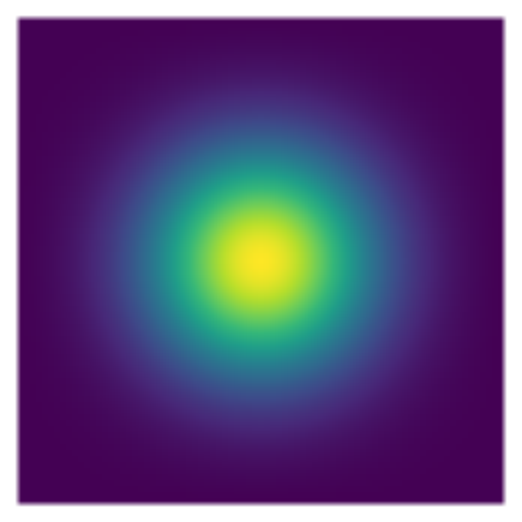
\includegraphics[width=\linewidth]{fig_harmonic2d_net.png}
  \caption{harmonic, network}
\end{subfigure}\hfill
\begin{subfigure}{0.31\linewidth}
  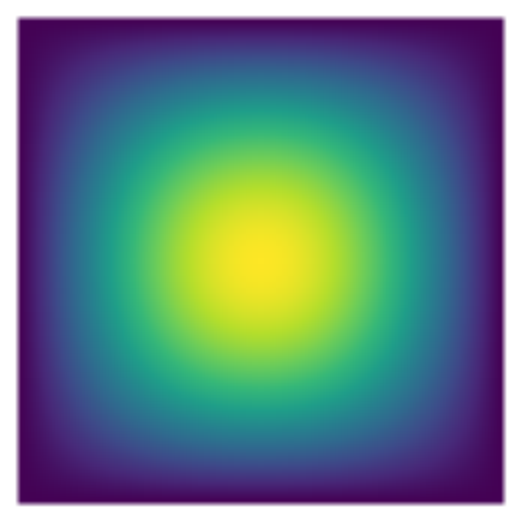
\includegraphics[width=\linewidth]{fig_well2d_net.png}
  \caption{box, network}
\end{subfigure}\hfill
\begin{subfigure}{0.31\linewidth}
  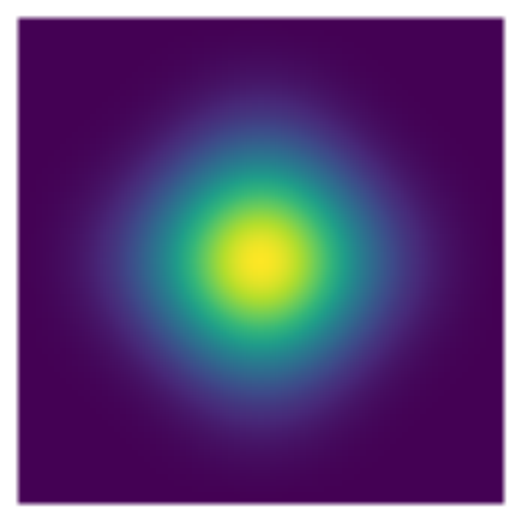
\includegraphics[width=\linewidth]{fig_anharmonic2d_net.png}
  \caption{anharmonic, network}
\end{subfigure}

\vspace{2pt}
\begin{subfigure}{0.31\linewidth}
  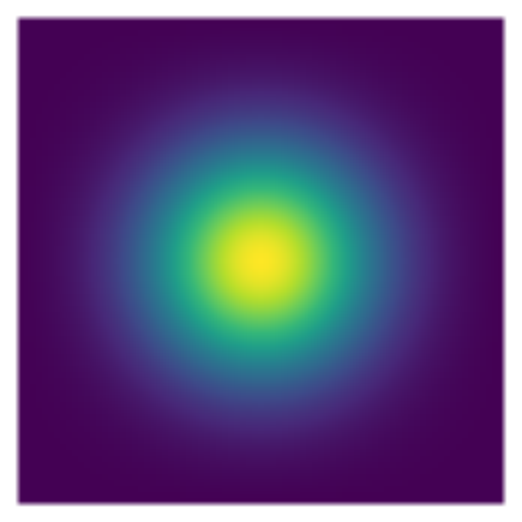
\includegraphics[width=\linewidth]{fig_harmonic2d_ref.png}
  \caption{harmonic, reference}
\end{subfigure}\hfill
\begin{subfigure}{0.31\linewidth}
  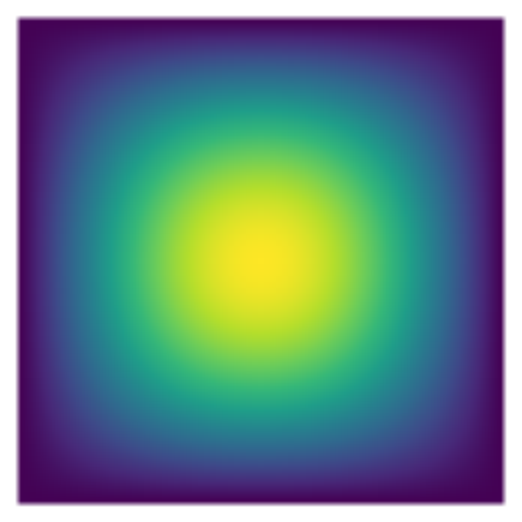
\includegraphics[width=\linewidth]{fig_well2d_ref.png}
  \caption{box, reference}
\end{subfigure}\hfill
\begin{subfigure}{0.31\linewidth}
  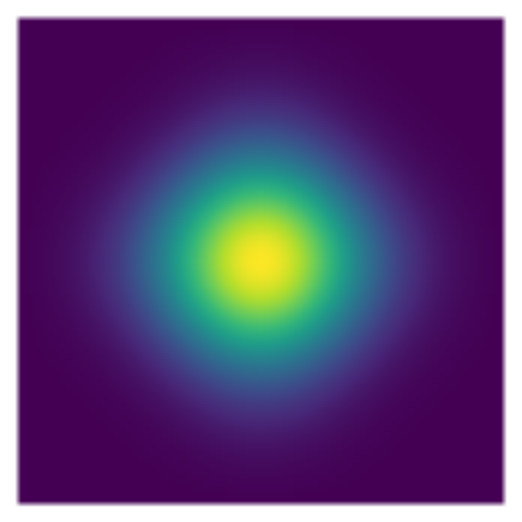
\includegraphics[width=\linewidth]{fig_anharmonic2d_ref.png}
  \caption{anharmonic, reference}
\end{subfigure}
\caption{Two-dimensional ground states: trained network (top) and discrete
reference (bottom), each normalised to its own maximum. Every reference field
is the ground eigenvector of the \emph{same} $\Hh$, returned by ARPACK on the
same grid; its eigenvalue agrees with the dense LAPACK values of
Table~\ref{tab:2d} to at least twelve digits. The reference is for display
only and enters no error estimate. Colour maps are linear in $|\psi|$.}
\label{fig:heatmaps}
\end{figure}

\subsection{Degenerate states are refused as states, certified as subspaces}
\label{sec:deg-results}

Table~\ref{tab:degeneracy} feeds \emph{exact} ARPACK eigenvectors of the box
potential into the single-state certificate. The ground state is certified with
width $2.0\times10^{-11}$. The first excited level is doubly degenerate: the
two eigenvalues differ by less than $2\times10^{-13}$ (round-off; the exact
value depends on the solver's start vector) and the eigenvectors are
$4\times10^{-12}$-accurate, yet the certificate refuses both of them and a
$0.43$ mixture.

\begin{table}[t]
\centering
\small
\setlength{\tabcolsep}{2pt}
\begin{tabular}{lccccc}
\toprule
Input state & $E$ & $r$ & certified & width & outcome \\
\midrule
Ground state & 9.868336 & $3.3\times10^{-12}$ & yes & $2.0\times10^{-11}$ & accepted \\
Excited (ARPACK 1) & 24.663232 & $4.3\times10^{-12}$ & no & -- & refused \\
Excited (ARPACK 2) & 24.663232 & $4.0\times10^{-12}$ & no & -- & refused \\
Excited (mixture) & 24.663232 & $4.8\times10^{-12}$ & no & -- & refused \\
\bottomrule
\end{tabular}

\caption{Degeneracy experiment on the $81\times81$ box. The verified gap for
the refused states is $7.1\times10^{-9}$, below the resolution floor
$1.3\times10^{-5}$ of \eqref{eq:floor}.}
\label{tab:degeneracy}
\end{table}

The refusal is the correct answer: no interval can contain exactly one of the
two eigenvalues, so neither \eqref{eq:temple} nor \eqref{eq:dk} has a
hypothesis, and the statement ``the state is identified'' is false even though
the residual is $10^{-12}$. The four rows make the point quantitatively: the residuals differ by less than
a factor of $1.5$ between the accepted ground state and the three refused
excited states, so a convention that reports residuals alone would rank them
as equally accurate, while the certificate's answer for the excited states is
that no eigenfunction is defined and nothing is certified. In a workflow that
ranks states or feeds them into a downstream calculation, that difference is
decisive.

\paragraph{The same data, certified as a subspace}
Table~\ref{tab:subspace} applies the cluster certificate of
Section~\ref{sec:subspace} to the same eigenspace. Given the two exact
eigenvectors the verified count returns $N(b)-N(a)=2$ on the interval
$(17.2658,\,32.0607)$, the Ritz residual is $\rho_F=6.1\times10^{-12}$ at the margin
$\delta=7.397$, and Theorem~\ref{thm:angle} bounds the angle to the
true invariant subspace by $8.2\times10^{-13}$, against a true angle of
$2.3\times10^{-16}$. The eigenvectors that ARPACK returns for a degenerate
level depend on its start vector, so the residual---and with it the last digit
of the bound---moves between runs ($8.2$--$8.5\times10^{-13}$); the verified
interval and the acceptance do not, and it is those that the certificate
asserts. The rotated basis $(x_1,\,0.6x_1+0.8x_2)$ returns the same
interval to all printed digits, which is the basis independence of the
symmetric orthogonalization; the certificate depends on $\operatorname{span}$
and not on how the columns were chosen. The refusals are equally
informative: one member of the pair alone ($m=1$) is refused because no
interval isolates it, and the set $\{\text{ground},\ \text{4th level}\}$ is
refused because any interval containing both of its Ritz values also
contains the degenerate pair, so the count is $4$, not $2$.
A subspace that skips a state is never reported as a smaller success.

\begin{table}[t]
\centering
\scriptsize
\setlength{\tabcolsep}{2pt}
\begin{tabular}{lccccccc}
\toprule
Input & $m$ & $N(b)\!-\!N(a)$ & $\rho_F$ & $\delta$ & $\Theta\le$ & $\Theta_{\mathrm{true}}$ & outcome \\
\midrule
Exact pair & 2 & 2 & $6.1\times10^{-12}$ & $7.4$ & $8.2\times10^{-13}$ & $2.3\times10^{-16}$ & accepted \\
Exact pair, rotated basis & 2 & 2 & $6.3\times10^{-12}$ & $7.4$ & $8.5\times10^{-13}$ & $3.0\times10^{-16}$ & accepted \\
One member ($m=1$) & 1 & -- & $4.4\times10^{-12}$ & -- & -- & -- & refused \\
Ground $+$ 4th level & 2 & -- & $5.7\times10^{-12}$ & -- & -- & -- & refused \\
\midrule
Networks 0, 1 & 2 & -- & $16.3$ & $6.08$ & -- & -- & refused \\
Networks 0, 2 & 2 & 2 & $4.6$ & $7.31$ & $0.68$ & $2.8\times10^{-2}$ & accepted \\
Networks 0, 3 & 2 & 2 & $4.1\times10^{-2}$ & $7.4$ & $5.6\times10^{-3}$ & $3.0\times10^{-4}$ & accepted \\
Networks 1, 2 & 2 & -- & $7.53$ & $7.18$ & -- & -- & refused \\
Networks 1, 3 & 2 & 2 & $4.5\times10^{-2}$ & $7.4$ & $6.1\times10^{-3}$ & $2.4\times10^{-4}$ & accepted \\
Networks 2, 3 & 2 & 2 & $4.7\times10^{-2}$ & $7.4$ & $6.3\times10^{-3}$ & $2.5\times10^{-4}$ & accepted \\
Seeds 0, 1, rotated & 2 & -- & $16.3$ & $6.08$ & -- & -- & refused \\
Seeds 0, 3, rotated & 2 & 2 & $4.1\times10^{-2}$ & $7.4$ & $5.6\times10^{-3}$ & $3.0\times10^{-4}$ & accepted \\
Network $+$ partner & 2 & 2 & $3.8\times10^{-2}$ & $7.4$ & $5.2\times10^{-3}$ & $2.8\times10^{-4}$ & accepted \\
Network $+$ mix, partner & 2 & 2 & $3.8\times10^{-2}$ & $7.4$ & $5.2\times10^{-3}$ & $2.8\times10^{-4}$ & accepted \\
\bottomrule
\end{tabular}

\caption{Cluster certificates on the $81\times81$ box. $m$ is the number of
vectors supplied, $N(b)-N(a)$ the \emph{verified} multiplicity (a dash when the
certificate refuses before the count is meaningful), $\rho_F$ the Frobenius
residual, $\delta$ the cluster margin \eqref{eq:margin}, $\Theta$ the
certified angle bound $\arcsin(\rho_F/\delta)$ and $\Theta_{\mathrm{true}}$ the
true principal angle, both in radians and the latter computed with a dense
reference. In the neural block,
runs 0, 1 and 2 converged to the same representative and run 3 to its partner;
the certificate accepts the pairs that contain run 3, refuses $(0,1)$ and
$(1,2)$, and accepts $(0,2)$ with a much weaker bound. The last two rows use a
direction forced by deflating the first output.}
\label{tab:subspace}
\end{table}

\paragraph{Where the boundary lies: resolution, not degeneracy}
Table~\ref{tab:resolution} replaces the question ``is this level degenerate?''
by a measurement. Adding the anisotropy $\lambda(x^2-y^2)$ to the box splits
the pair by $0.076\,\lambda$ with the mean energy unchanged to the printed
digits, and the certificate is applied to both members at thirteen values of
$\lambda$. The single-state certificate refuses every pair whose splitting
lies below the counting floor---including splittings of $10^{-7}$ and
$10^{-6}$, six orders of magnitude above round-off and separated by ARPACK
without difficulty---and accepts as soon as the splitting passes it: refused
at $\text{split}/\text{floor}=0.95$, accepted at $1.01$, a factor of $1.06$
between the two. The quantity compared with the floor is the verified gap,
and its value is set by the interval construction. Above the transition the
endpoints sit a tenth of the splitting inside each neighbour, so the gap is
$0.9\times$split; at the crossing that proposal cannot clear the floor, the
count-bisection fallback returns an endpoint at the neighbouring eigenvalue,
and the gap is the splitting itself---which is why acceptance begins exactly
at $\text{split}/\text{floor}=1$ rather than at $1/0.9$. The cluster
certificate, by contrast, accepts at every $\lambda$, exact degeneracy
included, with the same margin $\delta=7.397$ and a bound of
$7.4$--$9.8\times10^{-13}$: its margin is the distance to the next level, not
the internal splitting.

The practical content is that the phrase ``degenerate state'' is the wrong
category for this protocol. What decides certifiability is whether two shifts
can be separated in floating point, and a level split by $10^{-6}$ is as
uncertifiable as one split by $10^{-13}$. A practitioner who reports a pair of
near-degenerate states separately, with a validated interval each, cannot
support that claim on this grid; the pair as a subspace is certified to
$8\times10^{-13}$ in the same run.

\begin{table}[t]
\centering
\footnotesize
\setlength{\tabcolsep}{2pt}
\begin{tabular}{lcccccc}
\toprule
$\lambda$ & split $|E_1-E_2|$ & floor & split/floor & single state & $\delta$ & $\Theta\le$ \\
\midrule
$0$ & $<10^{-12}$ & $1.3\times10^{-5}$ & $<0.01$ & refused & $7.4$ & $8.4\times10^{-13}$ \\
$1.0\times10^{-5}$ & $7.6\times10^{-7}$ & $1.3\times10^{-5}$ & $0.06$ & refused & $7.4$ & $7.5\times10^{-13}$ \\
$3.0\times10^{-5}$ & $2.3\times10^{-6}$ & $1.3\times10^{-5}$ & $0.18$ & refused & $7.4$ & $8.7\times10^{-13}$ \\
$1.0\times10^{-4}$ & $7.6\times10^{-6}$ & $1.3\times10^{-5}$ & $0.59$ & refused & $7.4$ & $8.1\times10^{-13}$ \\
$1.5\times10^{-4}$ & $1.1\times10^{-5}$ & $1.3\times10^{-5}$ & $0.89$ & refused & $7.4$ & $7.6\times10^{-13}$ \\
$1.6\times10^{-4}$ & $1.2\times10^{-5}$ & $1.3\times10^{-5}$ & $0.95$ & refused & $7.4$ & $7.6\times10^{-13}$ \\
$1.7\times10^{-4}$ & $1.3\times10^{-5}$ & $1.3\times10^{-5}$ & $1.01$ & accepted & $7.4$ & $8.1\times10^{-13}$ \\
$1.9\times10^{-4}$ & $1.4\times10^{-5}$ & $1.3\times10^{-5}$ & $1.13$ & accepted & $7.4$ & $7.6\times10^{-13}$ \\
$2.0\times10^{-4}$ & $1.5\times10^{-5}$ & $1.3\times10^{-5}$ & $1.19$ & accepted & $7.4$ & $7.4\times10^{-13}$ \\
$3.0\times10^{-4}$ & $2.3\times10^{-5}$ & $1.3\times10^{-5}$ & $1.78$ & accepted & $7.4$ & $7.7\times10^{-13}$ \\
$4.0\times10^{-4}$ & $3.0\times10^{-5}$ & $1.3\times10^{-5}$ & $2.37$ & accepted & $7.4$ & $9.8\times10^{-13}$ \\
$1.0\times10^{-3}$ & $7.6\times10^{-5}$ & $1.3\times10^{-5}$ & $5.94$ & accepted & $7.4$ & $8.3\times10^{-13}$ \\
$1.0\times10^{-2}$ & $7.6\times10^{-4}$ & $1.3\times10^{-5}$ & $59.37$ & accepted & $7.4$ & $8.2\times10^{-13}$ \\
\bottomrule
\end{tabular}

\caption{Resolution boundary on the $81\times81$ box perturbed by
$\lambda(x^2-y^2)$, which splits the level linearly with the mean energy
unchanged. ``floor'' is $10^{-9}s$ of \eqref{eq:floor}. The single-state
certificate accepts when the verified gap passes the floor; the gap is nine
tenths of the splitting above the transition and equal to it at the crossing,
so acceptance begins at $\text{split}/\text{floor}\approx1$. The cluster
certificate has no such transition. Widths are
omitted because the two-sided enclosure of an exact eigenvector is at the
round-off floor ($4.9\times10^{-11}$) in every accepted row.}
\label{tab:resolution}
\end{table}

\paragraph{Independent runs: which sets span the level?}
Four additional runs, initialised differently and each deflated against the
certified ground state, all reach the excited level: their energies agree with
the discrete eigenvalue $24.663232$ to $4.1\times10^{-6}$, their residuals lie
in $2.7$--$3.4\times10^{-2}$, every one is refused by the single-state
certificate (verified gap $3.8$--$4.1\times10^{-6}$, below the counting floor),
and every one lies in the exact eigenspace (fraction of its norm
$\ge0.99999996$). They are nevertheless not four independent directions. Runs
0, 1 and 2 converged to the same representative---pairwise overlaps
$0.99996$--$0.999997$, mutual angles $0.14^\circ$--$0.52^\circ$---while run 3
converged to the orthogonal partner, with overlap $0.01$ with the others.
Whether a set of runs spans the level is therefore an empirical question with
no structural answer, and the certificate answers it for each set from the
vectors alone:
\begin{itemize}
\item $(0,1)$ is refused. The two outputs differ by $2.4\times10^{-3}$ in
  $L^2$, so the only second direction in their span is that difference, at
  grid scale; its Ritz residual is $16.25$, far above the margin $6.08$, and
  Lemma~\ref{lem:cluster} has no hypothesis to stand on. $(1,2)$ is refused
  for the same reason, at $\rho_F=7.53$ and $\delta=7.18$.
\item $(0,2)$ is accepted, but weakly: $\rho_F=4.60$ gives the bound $0.68$
  against a true angle of $0.028$. The certificate cannot know that this
  second direction is mostly noise; it can only report that the bound is two orders of
  magnitude looser than for a genuine pair---and it is still a valid bound.
\item $(0,3)$, $(1,3)$ and $(2,3)$ are accepted with
  $\rho_F=4.1$--$4.7\times10^{-2}$, $\delta=7.397$ and bounds
  $5.6$--$6.3\times10^{-3}$ against true angles of
  $2.4$--$3.0\times10^{-4}$.
\end{itemize}
No energy or residual separates these cases: the energies agree to
$4\times10^{-6}$ and the residuals lie in the same narrow band. Only the
subspace certificate does, and it orders the evidence the way a reader would.
Figure~\ref{fig:deg} shows the four functions behind the table: the two
symmetry-related representatives that the runs converged to, next to the two
exact modes they approximate.

\paragraph{A forced second direction}
When the goal is to certify the level rather than to test whether training
explored it, the second direction can be forced. Deflating the first network
output in addition to the ground state---the same projection that is applied
inside the loss---produces a function orthogonal to both (overlap
$10^{-18}$ with the first output), which still lies in the level:
$0.99999997$ of its norm is in the exact eigenspace, and it coincides with the
partner that run~3 found independently (overlap $0.99995$). The pair is
accepted with verified multiplicity $2$, $\rho_F=3.8\times10^{-2}$,
$\delta=7.397$ and an angle bound of $5.2\times10^{-3}$ against a true
principal angle of $2.8\times10^{-4}$. Rotating the basis
($0.6\psi_0+0.8\psi_\perp$ in place of $\psi_\perp$) leaves the interval, the
multiplicity and the bound unchanged, as it must: the object certified is the
subspace.

\begin{figure}[t]
\centering
\begin{subfigure}{0.24\linewidth}
  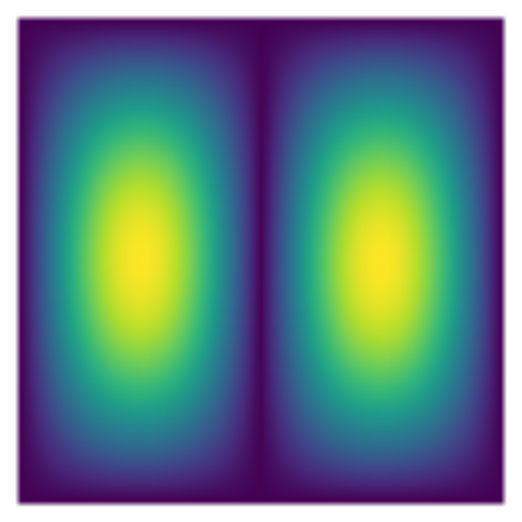
\includegraphics[width=\linewidth]{fig_deg_net_a.png}
  \caption{network, seed 0}
\end{subfigure}\hfill
\begin{subfigure}{0.24\linewidth}
  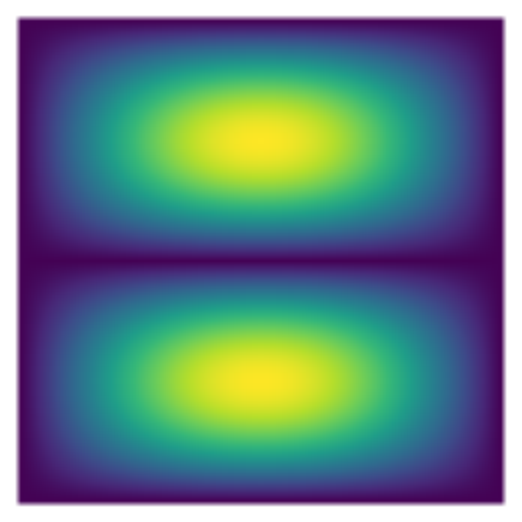
\includegraphics[width=\linewidth]{fig_deg_net_b.png}
  \caption{network, seed 3}
\end{subfigure}\hfill
\begin{subfigure}{0.24\linewidth}
  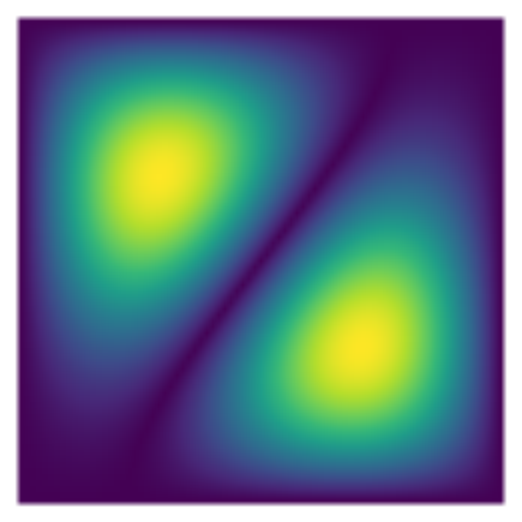
\includegraphics[width=\linewidth]{fig_deg_exact_a.png}
  \caption{exact, $\sin\pi x\sin2\pi y$}
\end{subfigure}\hfill
\begin{subfigure}{0.24\linewidth}
  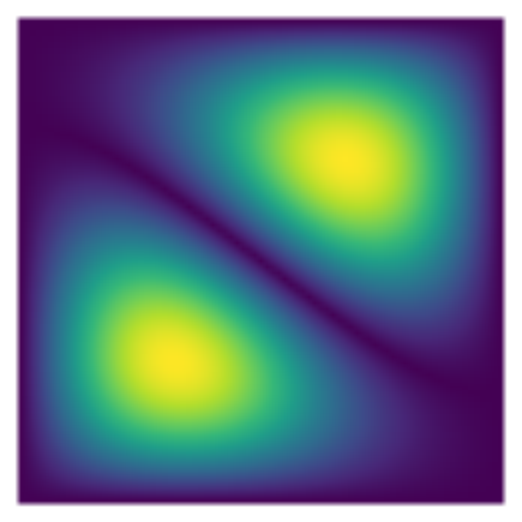
\includegraphics[width=\linewidth]{fig_deg_exact_b.png}
  \caption{exact, $\sin2\pi x\sin\pi y$}
\end{subfigure}
\caption{The doubly degenerate first excited level of the box, $|\psi|$ on the
$81\times81$ grid, each panel normalised to its own maximum. The two network
outputs are independent runs against the deflated ground state: one collapsed
onto the representative found by three of the four runs, the other onto its
orthogonal partner. They are visibly different functions---the nodal lines of
one are the reflections of the other's---and they span the same eigenspace to
within the certified angle.}
\label{fig:deg}
\end{figure}

The practical lesson is not that degenerate states are hard to train: all
four runs reached the level to $4\times10^{-6}$ in energy, and any of them
would pass a residual-based test. It is that the quantities such a run
reports---residual, energy, overlap with a chosen reference---are basis
dependent at a degenerate level, and that whether a set of outputs spans the
level is visible in none of them. The cluster certificate makes that question
decidable: it accepts the spanning pairs with a bound, refuses the collapsed
pair with a reason, and prices the difference between them in the bound
itself. A degenerate level can therefore be certified without a reference
solution, provided the dimension of the trial subspace is measured rather than
assumed.

\subsection{The discretization gap}
\label{sec:discretization}

Because the certificate refers to $\Hh$, its width bounds the error against
the discrete eigenvalue only; the distance to the continuous eigenvalue is a
separate quantity, bounded from above by the variational principle of
Section~\ref{sec:variational} and tabulated there. The two are independent:
the box width below is $2\times10^{-11}$ while the discretization error at the
same grid is $1.3\times10^{-3}$. Table~\ref{tab:disc}
quantifies that distance for the two potentials whose truncated-domain
eigenvalue can be extrapolated, using verified count bisection at five grids;
the extrapolated value $\lambda^\ast$ agrees with the variational bracket of
Table~\ref{tab:continuous} at the corresponding grid, which is the check that
the two independently computed descriptions of the same gap are consistent.

\begin{table}[t]
\centering
\small
\footnotesize
\setlength{\tabcolsep}{2.5pt}
\begin{tabular}{lcccccc}
\toprule
Pot.\ & $41$ & $61$ & $81$ & $101$ & $121$ & $\lambda^\ast$ \\
\midrule
Harmonic (2D) & $1.4\times10^{-3}$ & $6.2\times10^{-4}$ & $3.5\times10^{-4}$ & $2.2\times10^{-4}$ & $1.5\times10^{-4}$ & 1.0007826 \\
Box (2D) & $5.1\times10^{-3}$ & $2.3\times10^{-3}$ & $1.3\times10^{-3}$ & $8.1\times10^{-4}$ & $5.6\times10^{-4}$ & 9.8696042 \\
\bottomrule
\end{tabular}

\caption{Discretization error $|\lambda_h-\lambda^\ast|$ of the first
eigenvalue of $\Hh$; column headers are the grid size $N$ and
$\lambda^\ast$ is fitted from $\lambda(h)=\lambda^\ast+ch^2$. The
least-squares slope of $\log|\lambda_h-\lambda^\ast|$ against $\log h$ is
$2.00$ for both potentials.}
\label{tab:disc}
\end{table}

Two features deserve comment. The box potential extrapolates to
$\lambda^\ast=9.8696042046$, within $2.0\times10^{-7}$ of $\pi^2$, with a
clean second-order convergence; this is an end-to-end check of the counting,
bisection and extrapolation chain. The harmonic potential is subtler: its
infinite-domain eigenvalue is $1$, but the Dirichlet problem on the truncated
box $[-3,3]^2$ has eigenvalue $\lambda^\ast=1.0007826$, higher by
$7.8\times10^{-4}$ because the Gaussian tail is cut off. Consequently the raw
error against the analytic value $1$ \emph{increases} with $N$
($1.7\times10^{-4}$ at $N=61$ to $6.3\times10^{-4}$ at $N=121$) while the true
discretization error decreases at second order. Reporting only the first
column would look like a bug; reporting only the second would hide the
truncation. Both are needed, and the certificate makes the distinction
unavoidable.

At $N=81$ the harmonic discretization error against $\lambda^\ast$ is
$3.5\times10^{-4}$, three to eight times larger than the certified width of
the trained network ($0.5$--$1.1\times10^{-4}$). On this grid the network is
already better than the grid, and the certificate correctly reports the grid's
limitation rather than the network's.

\subsection{How tight is the enclosure?}
\label{sec:tightness}

Figure~\ref{fig:scatter} plots the certified width against the true error for
all 18 runs, together with the lines width $=10^{k}\times$ error. Across the
whole set the certified width lies between $5$ and $3\times10^{3}$ times the
true error, with a median ratio of $45$ over all 18 runs ($1.4\times10^{2}$
over the nine one-dimensional runs, $34$ over the two-dimensional ones). The
spread follows the potential rather than the dimension: $5$--$36$ on the
harmonic and anharmonic problems, $50$--$3\times10^{2}$ on the infinite well,
and $7\times10^{2}$--$3\times10^{3}$ on the finite well and the box. The two
large groups are large for different reasons. On the infinite well and the box
both the width and the error have reached the round-off floor
($9.9\times10^{-12}$ against $10^{-13}$ in one dimension, $2.0\times10^{-11}$
against $2.5\times10^{-14}$ in two), so the ratio is a ratio of round-off and
says nothing about the method; on the finite well neither quantity is at
round-off and the enclosure is genuinely wide, because the residual cannot
distinguish a high-wavenumber error from a genuine component of the same shape
(Section~\ref{sec:discussion}). For comparison, the same certificate applied to a
classical LAPACK eigenvector of the same $\Hh$ gives widths of
$2.0\times10^{-12}$ (harmonic), $9.9\times10^{-12}$ (infinite well) and
$9.8\times10^{-11}$ (finite well), saved by
\texttt{scripts/lapack\_reference\_widths.py} in
\url{runs/reference1d/lapack_certificates.json}: the machinery itself is not the limitation,
and a trained network's certified width is seven to ten orders of magnitude
wider on the harmonic and finite-well potentials. The infinite well is the
exception that proves the rule---after filtering, the network output is a
single sine mode, so its certificate sits at the same round-off floor as the
classical eigenvector's.

\begin{figure}[t]
\centering
\begin{tikzpicture}
\begin{axis}[
  width=0.62\linewidth, height=0.55\linewidth,
  xmode=log, ymode=log,
  xlabel={$|E_f-\lambda_h|$}, ylabel={certified width},
  xmin=1e-14, xmax=1e-2, ymin=1e-13, ymax=1e1,
  legend style={font=\footnotesize, at={(0.02,0.98)}, anchor=north west},
  grid=major, grid style={gray!25},
]
\addplot[only marks, mark=*, mark size=1.6pt, blue]
  table[col sep=comma,x=dE,y=width] {figures/data/scatter_1D_harmonic.csv};
\addplot[only marks, mark=square*, mark size=1.6pt, red!70!black]
  table[col sep=comma,x=dE,y=width] {figures/data/scatter_1D_finite_well.csv};
\addplot[only marks, mark=triangle*, mark size=2.2pt, green!50!black]
  table[col sep=comma,x=dE,y=width] {figures/data/scatter_1D_infinite_well.csv};
\addplot[only marks, mark=diamond*, mark size=2.2pt, orange!80!black]
  table[col sep=comma,x=dE,y=width] {figures/data/scatter_2D_harmonic2d.csv};
\addplot[only marks, mark=pentagon*, mark size=2.2pt, purple]
  table[col sep=comma,x=dE,y=width] {figures/data/scatter_2D_anharmonic2d.csv};
\addplot[only marks, mark=o, mark size=2.2pt, cyan!70!black]
  table[col sep=comma,x=dE,y=width] {figures/data/scatter_2D_well2d.csv};
\addplot[domain=1e-14:1e-2, dashed, black!60] {x};
\addplot[domain=1e-14:1e-4, dashed, black!35] {100*x};
\addplot[domain=1e-14:1e-6, dashed, black!20, forget plot] {10000*x};
\legend{1D harmonic, 1D finite well, 1D infinite well,
        2D harmonic, 2D anharmonic, 2D box}
\end{axis}
\end{tikzpicture}
\caption{Certified width against true error. Dashed lines: width $=$ error,
$100\times$ error, $10^4\times$ error. The points at the far left are the
infinite-well and box runs, whose filtered states are exact sine modes; the
upper-right outliers are the finite well.}
\label{fig:scatter}
\end{figure}

The figure also shows where the enclosure is genuinely informative: for the
smooth harmonic and anharmonic potentials the ratio is $5$--$40$, which is
enough to certify that a network is accurate to, say, $10^{-4}$ without any
reference. For the finite well the ratio is $10^{3}$ and only the
containment statement survives.

\begin{figure}[t]
\centering
\begin{subfigure}{0.48\linewidth}
\begin{tikzpicture}
\begin{axis}[
  width=0.94\linewidth, height=0.78\linewidth,
  xmode=log, ymode=log,
  xlabel={cutoff $K$}, ylabel={certified width},
  legend style={font=\scriptsize, at={(0.02,0.98)}, anchor=north west},
  grid=major, grid style={gray!25},
]
\addplot[thick, blue, mark=*, mark size=1pt]
  table[col sep=comma,x=cutoff,y=width] {figures/data/width_vs_cutoff_harmonic.csv};
\addplot[thick, red!70!black, mark=square*, mark size=1pt]
  table[col sep=comma,x=cutoff,y=width] {figures/data/width_vs_cutoff_finite_well.csv};
\addplot[thick, green!50!black, mark=triangle*, mark size=1pt]
  table[col sep=comma,x=cutoff,y=width] {figures/data/width_vs_cutoff_infinite_well.csv};
\legend{harmonic, finite well, infinite well}
\end{axis}
\end{tikzpicture}
\caption{width vs.\ truncation order}
\end{subfigure}\hfill
\begin{subfigure}{0.48\linewidth}
\begin{tikzpicture}
\begin{axis}[
  width=0.94\linewidth, height=0.78\linewidth,
  xmode=log, ymode=log,
  xlabel={$h$}, ylabel={$|\lambda_h-\lambda^\ast|$},
  legend style={font=\scriptsize, at={(0.5,0.03)}, anchor=south},
  grid=major, grid style={gray!25},
]
\addplot[thick, blue, mark=*, mark size=1.2pt]
  table[col sep=comma,x=h,y=error] {figures/data/conv2d_harmonic2d.csv};
\addplot[thick, red!70!black, mark=square*, mark size=1.2pt]
  table[col sep=comma,x=h,y=error] {figures/data/conv2d_well2d.csv};
\addplot[dashed, black!45, domain=0.008:0.16] {8.1*x^2};
\legend{harmonic (2D), box (2D), $8.1\,h^2$}
\end{axis}
\end{tikzpicture}
\caption{discretization error vs $h$}
\end{subfigure}
\caption{(a) Certified width against the DST truncation order for one run
per potential; the minimum is what the protocol selects
without a reference. (b) Discretization error of the two-dimensional ground
states against the $h\to0$ limit; the dashed line is the expected second-order
slope.}
\label{fig:filter}
\end{figure}
